\documentclass[letterpaper,12pt]{article}

\usepackage[utf8]{inputenc}
\usepackage{amsmath}
\usepackage{amssymb}
\usepackage{graphicx}
\usepackage{hyperref}
\usepackage{geometry}
\usepackage{fancyhdr}
\usepackage{booktabs}
\usepackage{float}
\usepackage{titling}
\usepackage{multicol}
\usepackage{subcaption}
\graphicspath{ {./images/} }

\geometry{margin=0.5in}
% Adjust the vertical space above the title
\setlength{\droptitle}{-5em} % Reduce as needed

\pagestyle{fancy}
\fancyhf{}
% Customize title spacing and font size
\pretitle{\begin{center}\Large}
\posttitle{\par\end{center}\vspace{-2ex}}

\preauthor{\begin{center}\small}
\postauthor{\end{center}\vspace{-2ex}}

\predate{\begin{center}\small}
\postdate{\end{center}\vspace{-2ex}}

\title{Sim4Life Frequency Modulation Report}
\author{Sam Tran}
\date{\today}

\begin{document}
\maketitle
\section*{Method}

\noindent Given the following function to calculate threshold intensity (voltage):
\begin{equation}
    V_{threshold} = \phi \cdot T \cdot a(t)
\end{equation}
where:
\begin{itemize}
    \item $V_{threshold}$ is the threshold intensity in voltage. This is the value we are trying to find.
    \item $\phi$ is the stimulated voltage. We keep this value equal to 1 $V_{pp}$ going from -0.5 $V$ to 0.5 $V$
    \item $a(t)$ is the intensity of the modulated signal. We vary this value between two values, 10$V$ and 20$V$, to keep the titration factor as close to 1 as possible. 
    \item $T$  is the titration factor. This value is calculated by the simulation by adjusting the sensitivity of the signal until an action potential is produced.
\end{itemize}

\noindent The chosen sets of parameters for the simulation are:
\begin{table}[H]
    \centering
    \scriptsize
    \begin{minipage}[t]{0.45\textwidth}
    \centering
    % First half of the table
    \begin{tabular}{|c|c|c|}
    \toprule
    \textbf{$a(t)$} & \textbf{$Frequency (Hz)$} & \textbf{$\phi (V)$} \\
    \midrule
    20 & 20   & 1 \\
    20 & 40   & 1 \\
    20 & 60   & 1 \\
    10 & 80   & 1 \\
    10 & 160  & 1 \\
    20 & 240  & 1 \\
    10 & 320  & 1 \\
    10 & 480  & 1 \\
    10 & 640  & 1 \\
    \bottomrule
    \end{tabular}
    \caption{Parameter Sets 1}
    \end{minipage}\hfill
    % Second half of the table
    \begin{minipage}[t]{0.45\textwidth}
    \centering
    \begin{tabular}{|c|c|c|}
    \toprule
    \textbf{$a(t)$} & \textbf{$Frequency (Hz)$} & \textbf{$\phi (V)$} \\
    \midrule
    20 & 800  & 1 \\
    10 & 1200 & 1 \\
    10 & 1500 & 1 \\
    10 & 1700 & 1 \\
    10 & 3000 & 1 \\
    10 & 6000 & 1 \\
    10 & 1200 & 1 \\
    10 & 2400 & 1 \\
    \bottomrule
    \end{tabular}
    \caption{Parameter Sets 2}
    \end{minipage}
\end{table}
\noindent Other settings of the simulation source are:
\begin{multicols}{2}
\begin{itemize}
    \item Pulse Type: Sinusoidal
    \item Frenquency: 20Hz to 24000Hz
    \item Amplitude: 10V or 20V
    \item Number Of Half Period Sine: 12kHz
    \item Solver Duration: $0.003s$
    \item Time Step: $0.0025ms$
    \item Initial Time: $0.0001s$
\end{itemize}
\end{multicols}

\noindent The three nerve fibers/axon chosen for this simulation along with nodes for placing point sensor are:
\begin{itemize}
    \item Dorsal root spinal C5 brachial plexus radial right (C5) at nodes 55, 112, and 140.
    \item Ventral root spinal C8 brachial plexus median right (C8) at nodes 60, 114, and 152.
    \item Ventral root spinal T1 brachial plexus ulnar right (T1) at nodes 60, 114, and 150.
\end{itemize}

\noindent The codes for sweeping different pairs of frequency and intensity and for generating this report are available in the following Github repository: \url{https://github.com/samsam2610/Sim4Life-Sweeping}

\section*{Result}
\noindent The following figures and tables show the example result at $24kHz$ and the full results of the simulations as pair of frequency and titration factor of an axon.
\begin{figure}[H]
    \centering
    \begin{subfigure}[b]{0.45\textwidth}
        \centering
        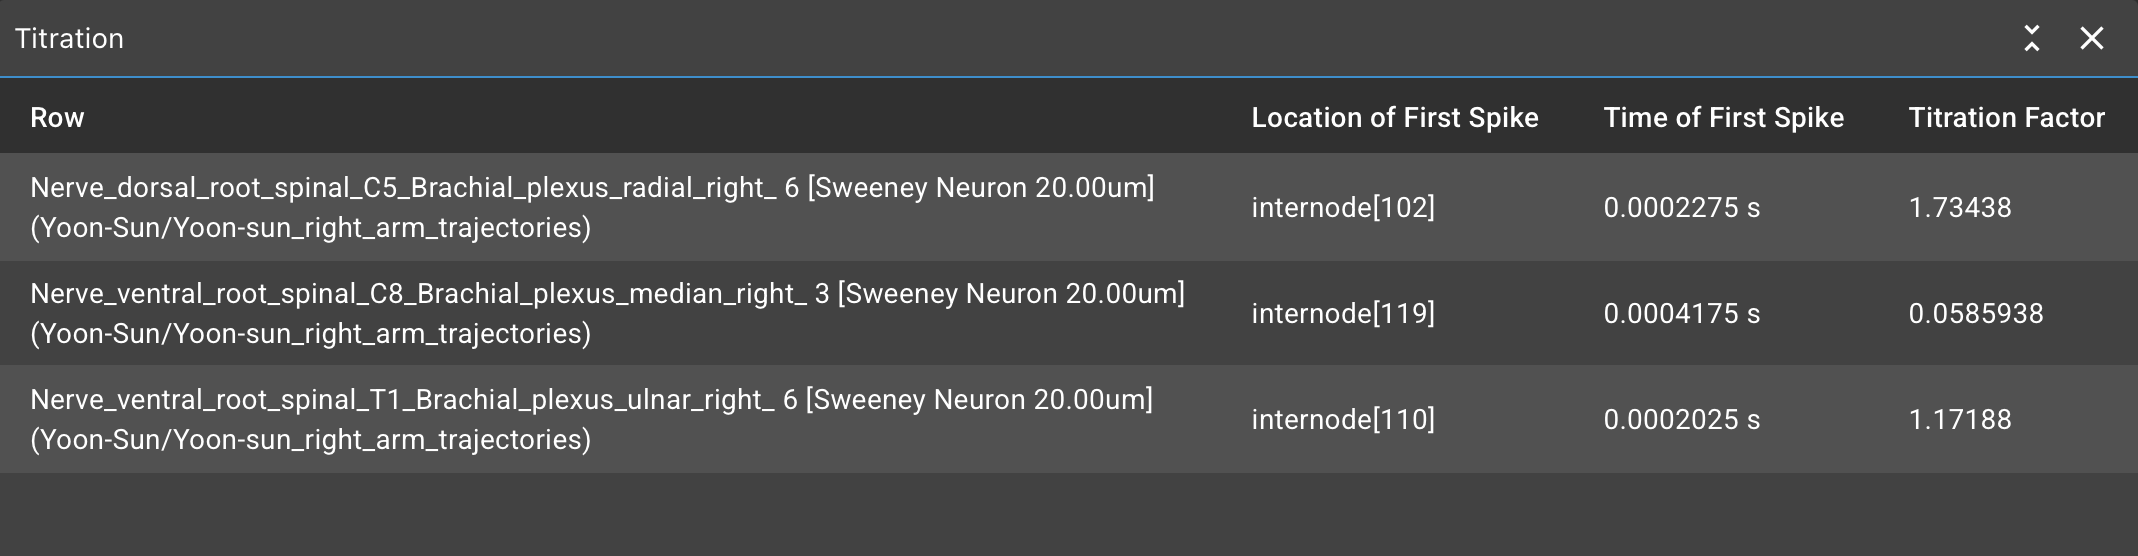
\includegraphics[scale=0.11]{titration_factor.png}
        \caption{Titration Factor of different axons} 
        \label{fig:titration}
    \end{subfigure}
    \vfill
    \begin{subfigure}[b]{0.45\textwidth}
        \centering
        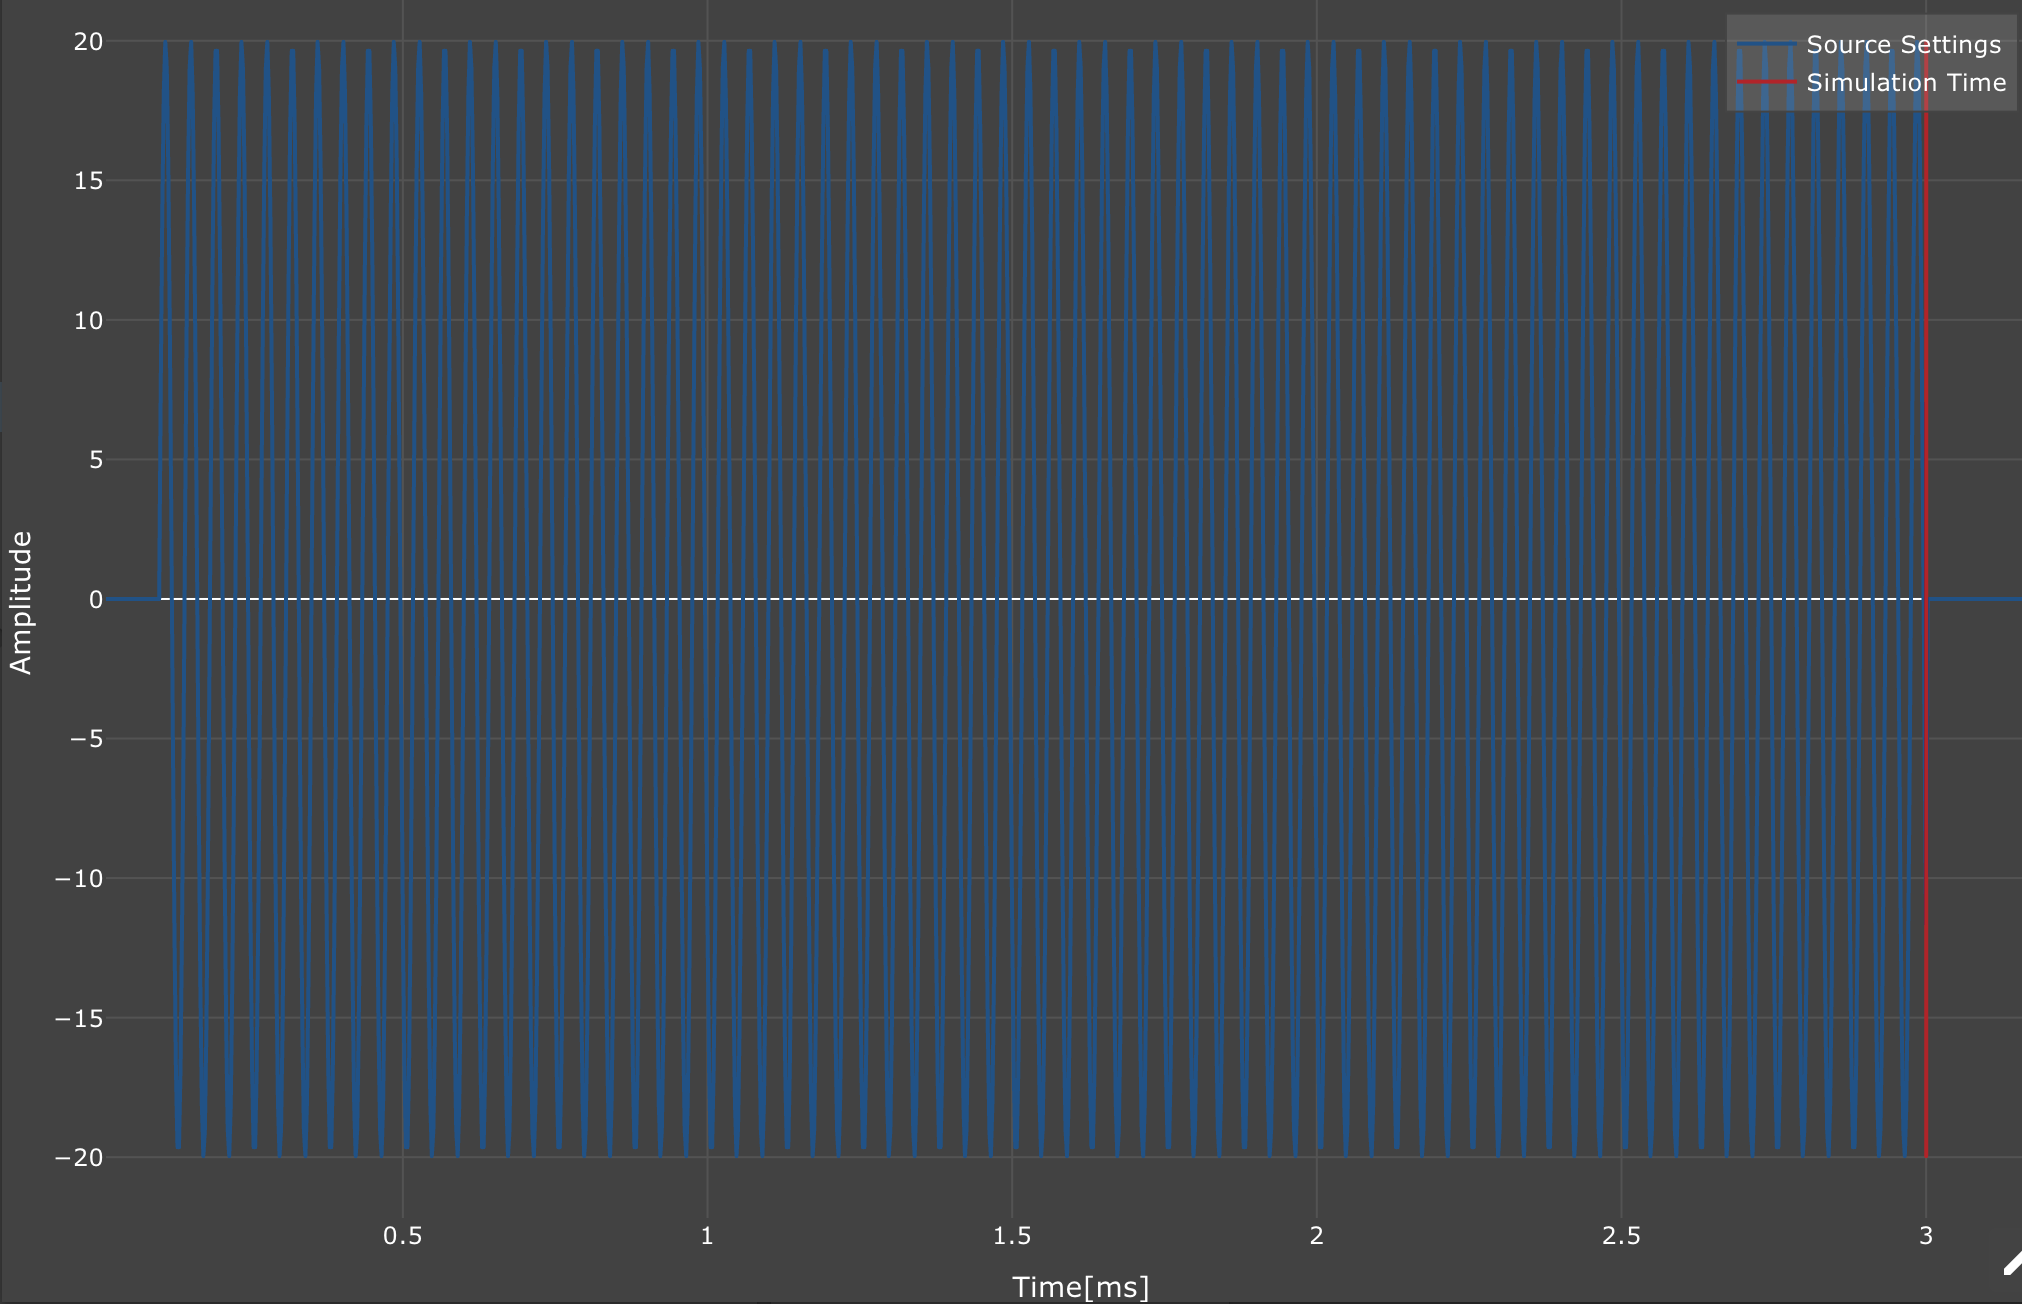
\includegraphics[scale=0.10]{source_signal.png}
        \caption{Plot of the source signal}
        \label{fig:source_signal}
    \end{subfigure}
    \hfill
    \begin{subfigure}[b]{0.45\textwidth}
        \centering
        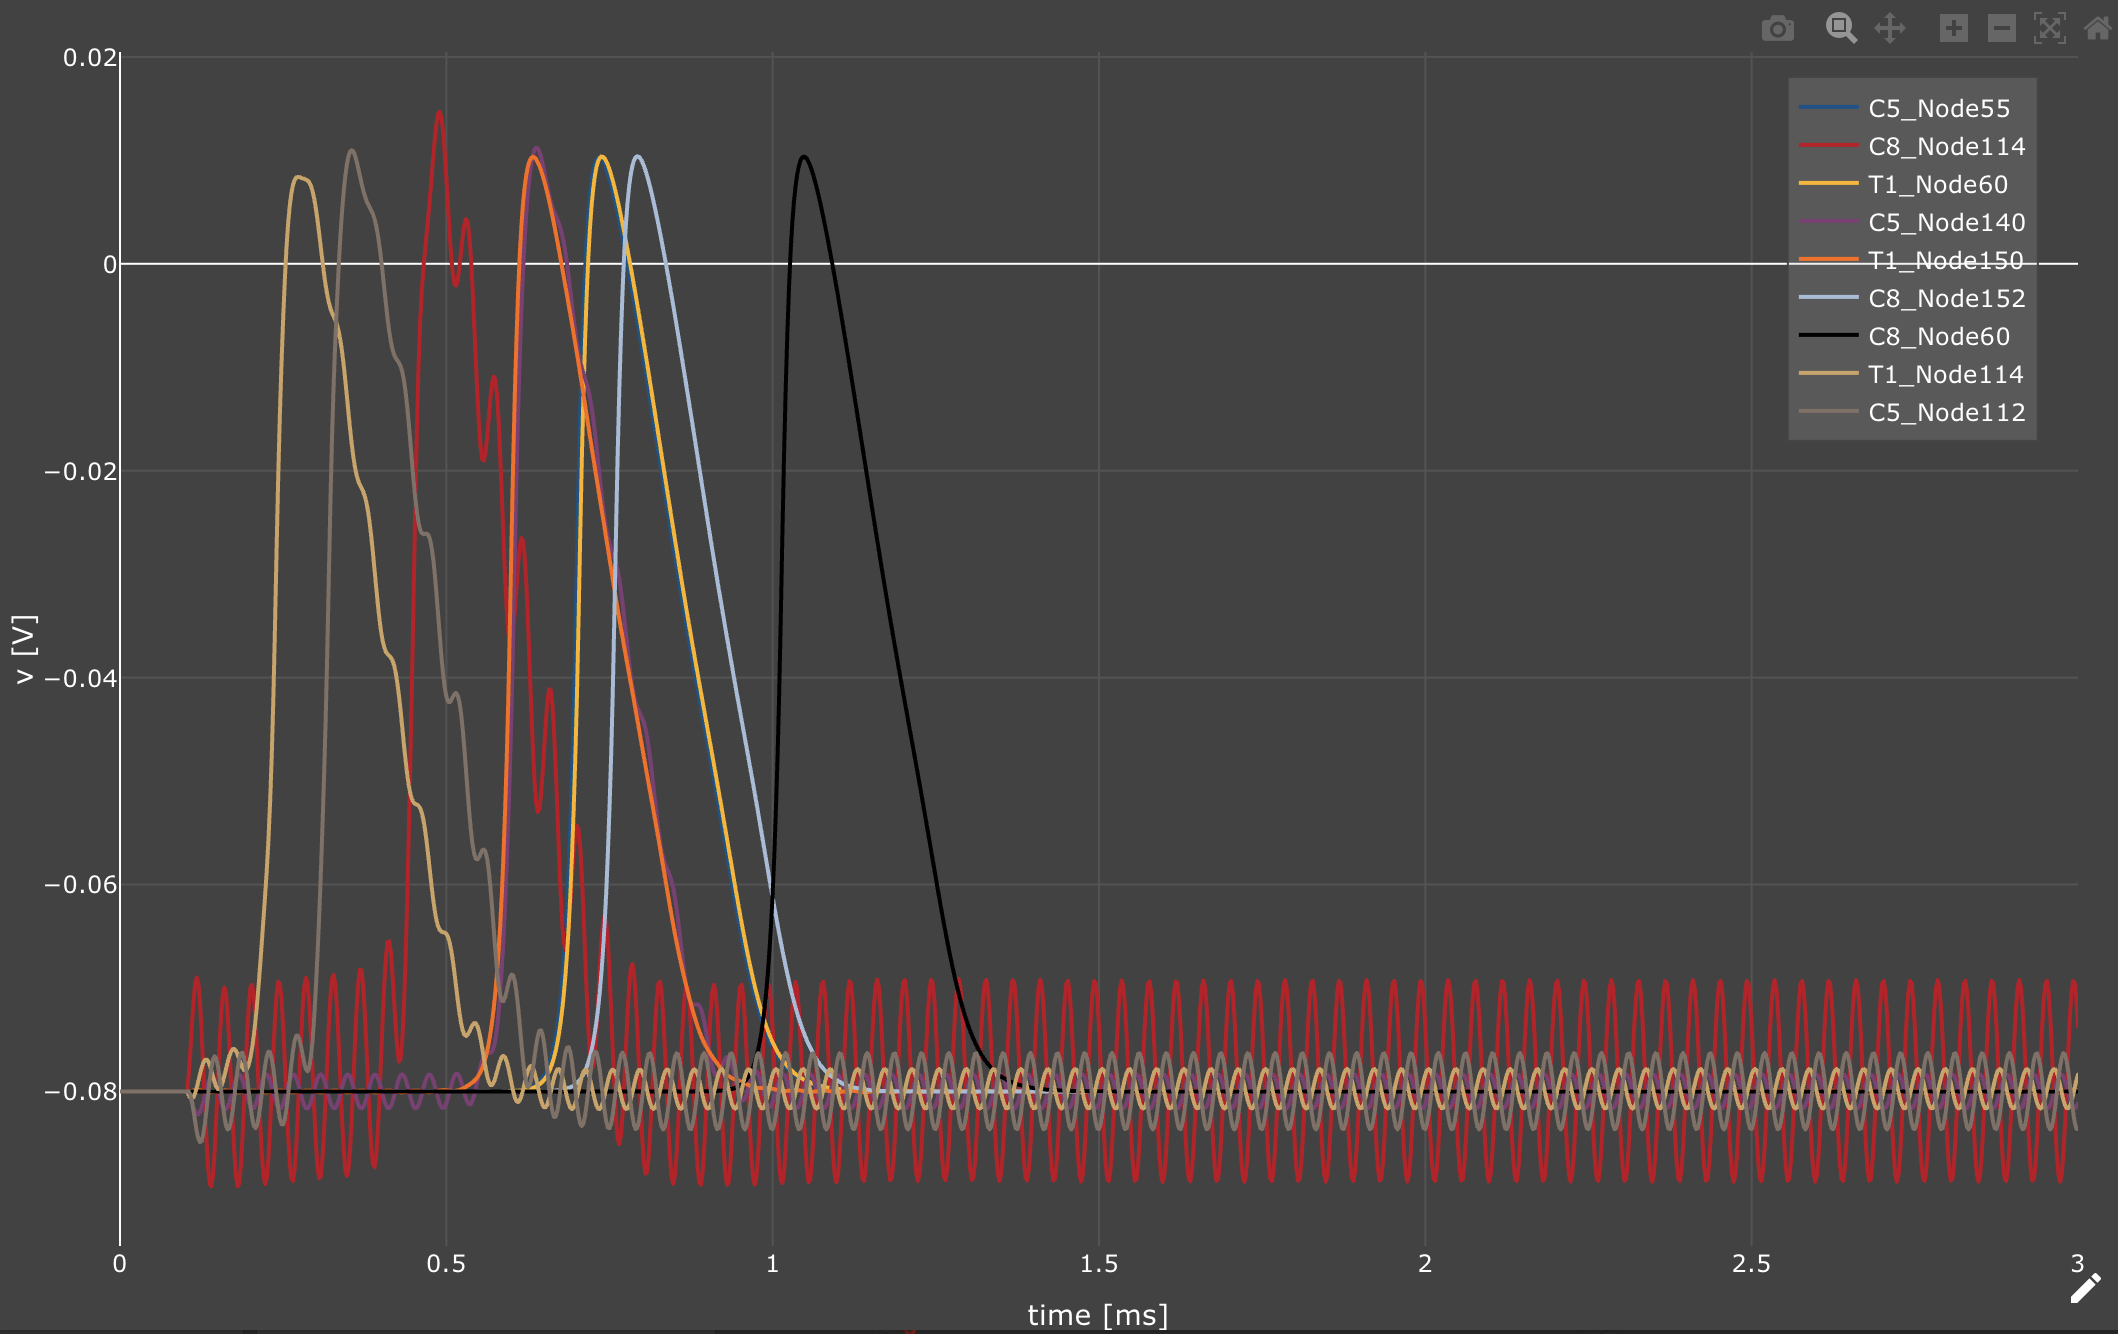
\includegraphics[scale=0.10]{action_potential_registered.png}
        \caption{Action Potential Registered at different nodes along the axons}
        \label{fig:action_potential}
    \end{subfigure}
    \caption{Example output of the simulation at $24kHz$.}
    \label{fig:combined}
\end{figure}

\begin{table}[H]
    \centering
    \scriptsize
    \begin{minipage}[t]{0.45\textwidth}
    \centering
    % First half of the table
    \begin{tabular}{|c|c|c|c|}
    \toprule
    \textbf{$Freq (Hz)$} & \textbf{$T_{C8}$} & \textbf{$T_{T1}$} & \textbf{$T_{C5}$} \\
    \midrule
    20	 &0.148438	 &1.125	     &1.84375 \\
    40	 &0.0800781	 &0.605469	 &1.02344 \\
    60	 &0.0595703	 &0.46875	 &0.789062 \\
    80	 &0.100586	 &0.84375	 &1.35938 \\
    160	 &0.0761719	 &0.710938	 &1.09375 \\
    240	 &0.0223389	 &0.330078	 &0.503906 \\
    320	 &0.0385742	 &0.632812	 &0.960938 \\
    480	 &0.0361328	 &0.597656	 &0.90625 \\
    640	 &0.0349121	 &0.582031	 &0.882812 \\
    \bottomrule
    \end{tabular}
    \caption{Outputs 1}
    \end{minipage}\hfill
    % Second half of the table
    \begin{minipage}[t]{0.45\textwidth}
    \centering
    \begin{tabular}{|c|c|c|c|}
    \toprule
    \textbf{$Freq (Hz)$} & \textbf{$T_{C8}$} & \textbf{$T_{T1}$} & \textbf{$T_{C5}$} \\
    \midrule
    800	    &0.0172119	&0.287109	&0.433594 \\
    1200	&0.0170898	&0.289062	&0.4375 \\
    1500	&0.017334	&0.292969	&0.441406 \\
    1700	&0.0174561	&0.296875	&0.449219 \\
    3000	&0.019043	&0.333984	&0.503906 \\
    6000	&0.0240479	&0.445312	&0.671875 \\
    12000	&0.0358887	&0.679688	&1.02344 \\
    24000	&0.0585938	&1.17188	&1.73438 \\
    \bottomrule
    \end{tabular}
    \caption{Outputs 2}
    \end{minipage}
\end{table}

\noindent By multiplying the titration factor by the stimulated voltage and the intensity of the modulated signal, we can calculate the threshold intensity in voltage required to trigger an action potential in the axon. The following plot shows the relationship between the frequency and the threshold intensity for each of the three axons.
\begin{figure}[H]
    \centering
    \includegraphics[scale=0.13]{{plotted_results_3.png}}
    \caption{Threshold Intensity vs Frequency}
\end{figure}

\end{document}